\documentclass[letterpaper,12pt]{article}
\usepackage{tabularx} % extra features for tabular environment
\usepackage{amsmath}  % improve math presentation
\usepackage{float}
\usepackage{pdfpages}
\usepackage{steinmetz}

\usepackage{graphicx} % takes care of graphic including machinery
\graphicspath{ {./figures/} }
\usepackage[margin=1in,letterpaper]{geometry} % decreases margins
\usepackage{cite} % takes care of citations
\usepackage[final]{hyperref} % adds hyper links inside the generated pdf file
\hypersetup{
	colorlinks=true,       % false: boxed links; true: colored links
	linkcolor=blue,        % color of internal links
	citecolor=blue,        % color of links to bibliography
	filecolor=magenta,     % color of file links
	urlcolor =blue         
}




\begin{document}

\title{Homework 3 Part 2 }
\author{Ahmet Akman 2442366 }
\date{\today}
\maketitle
%\begin{abstract}
%abstract
%\end{abstract}
\section{a)}
First, duty cycle increases then the load torque is increased. It is expected to have higher rotational speed as the terminal voltage increases with increasing duty cycle. For the increase in the load torque the expected behavior is to have a decrease in the rotational speed. For example the maximum rotational speed is obtained at the time interval of 12-14 seconds ,and minimum nonzero rotational speed is expected at time interval of 4-6 seconds. 
\section{b)}
The plot of currents are given in Figure \ref{currents}.

\begin{figure}[H]
    \centering
    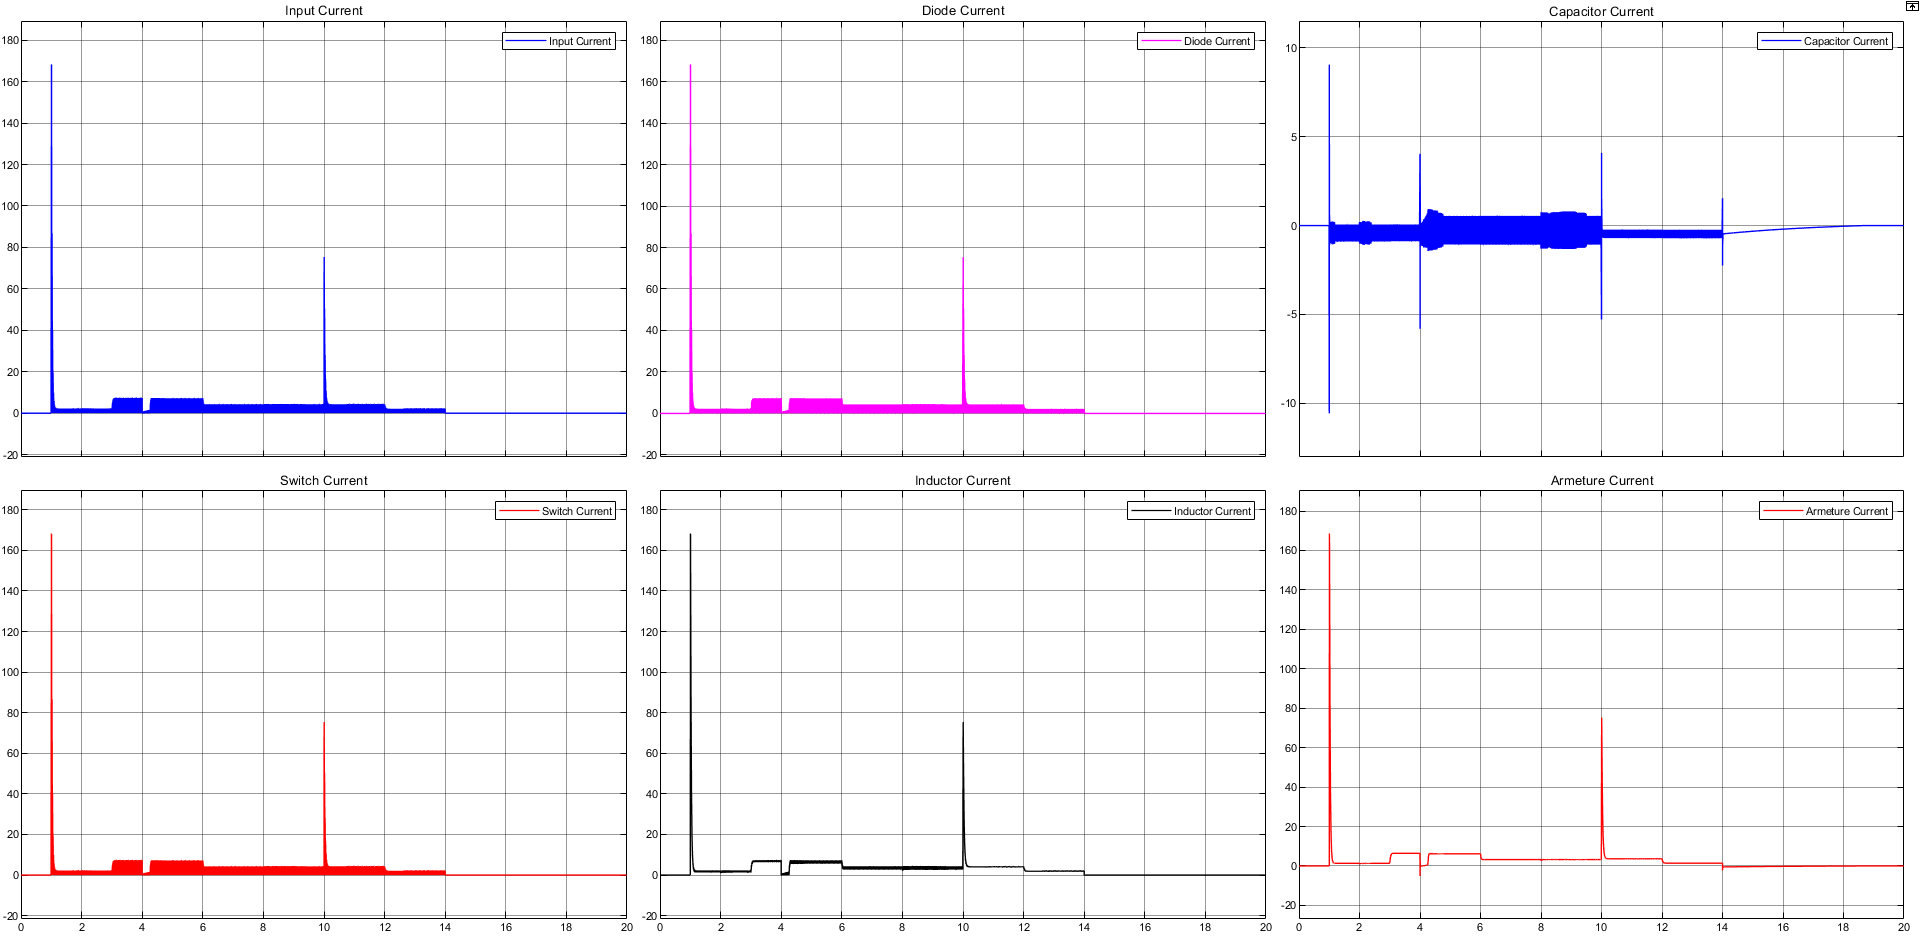
\includegraphics[width=1\textwidth]{case1_1.png}
    \caption{Current plots}
    \label{currents}
\end{figure} 
By looking at the plots it can be said that there occurs overshoots in the currents. These are caused because of the sudden changes in the duty cycle. So, the current transiently inceares to a very high value like a starters motors.
\section{c)}
The plot that shows the torque data with rotational speed is given in Figure \ref{torques}
\begin{figure}[H]
    \centering
    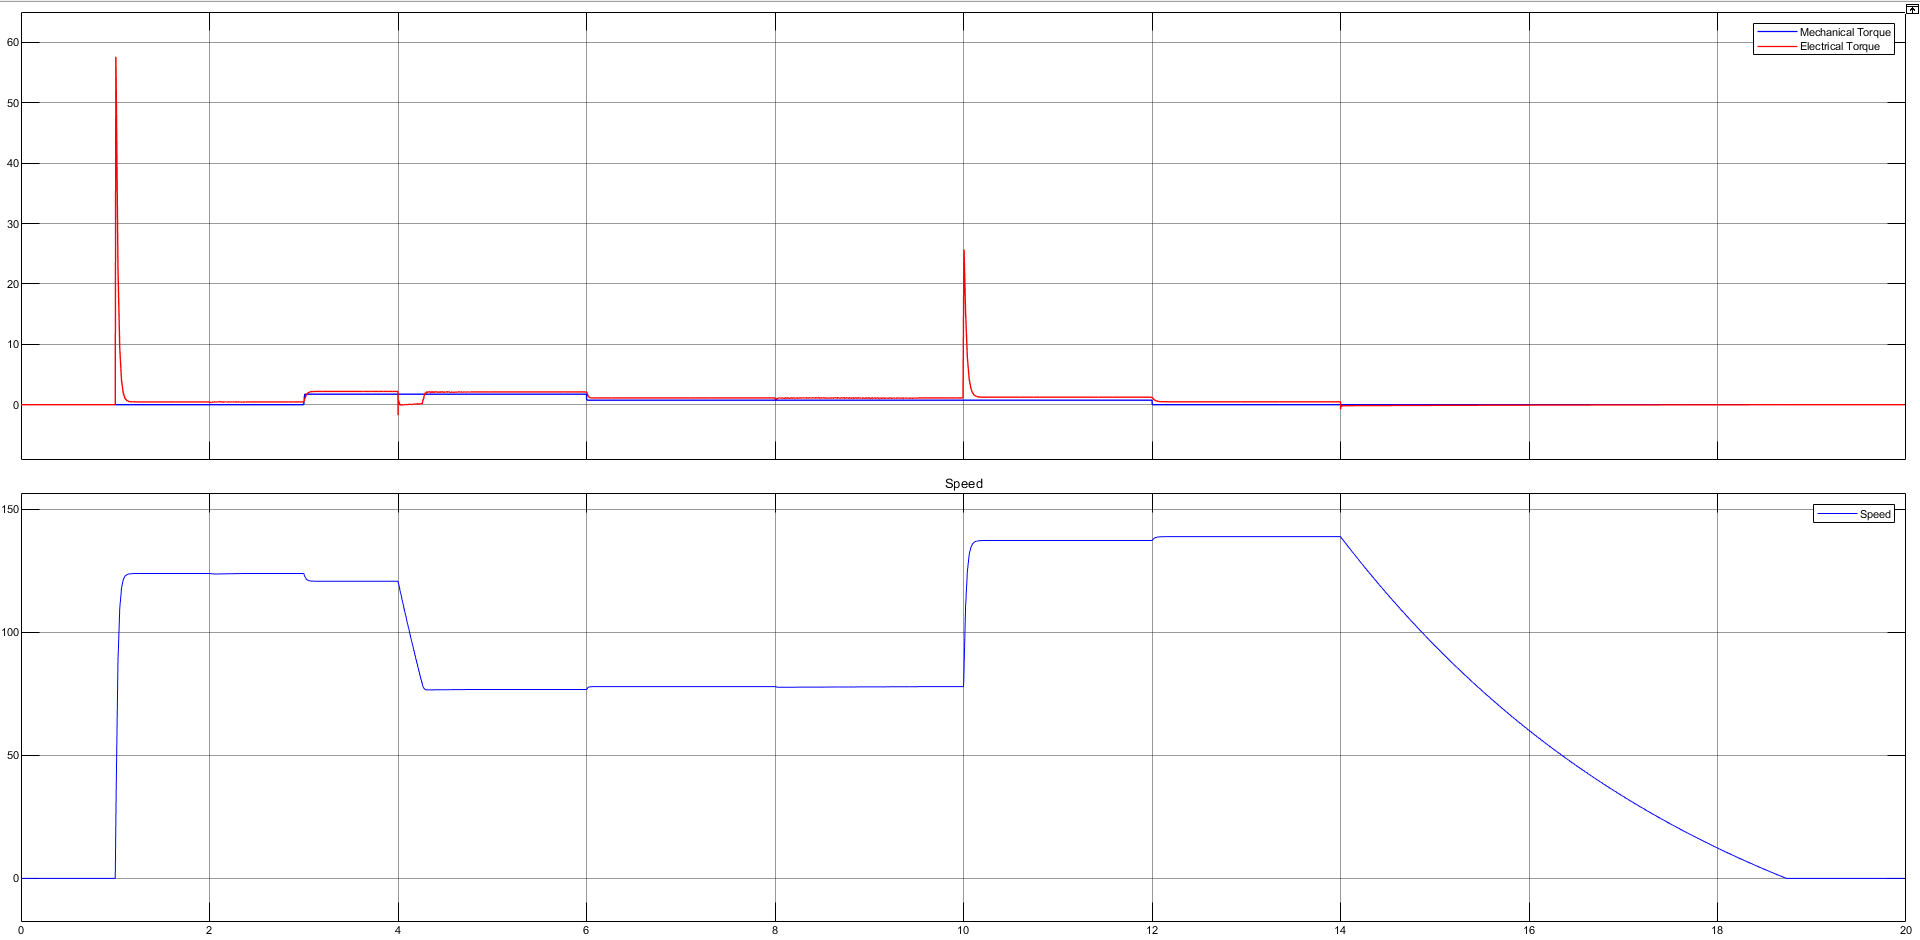
\includegraphics[width=1\textwidth]{case1_2_torque_speed.png}
    \caption{Torque and speed}
    \label{torques}
\end{figure} 
From the plot it can be said that speed is related through to the electrical and mechanical torque directly if we discard overshoots . 
\section{d)}
The plot that dectribes duty cycle with the input and terminal voltages is given in \ref{voltages}
\begin{figure}[H]
    \centering
    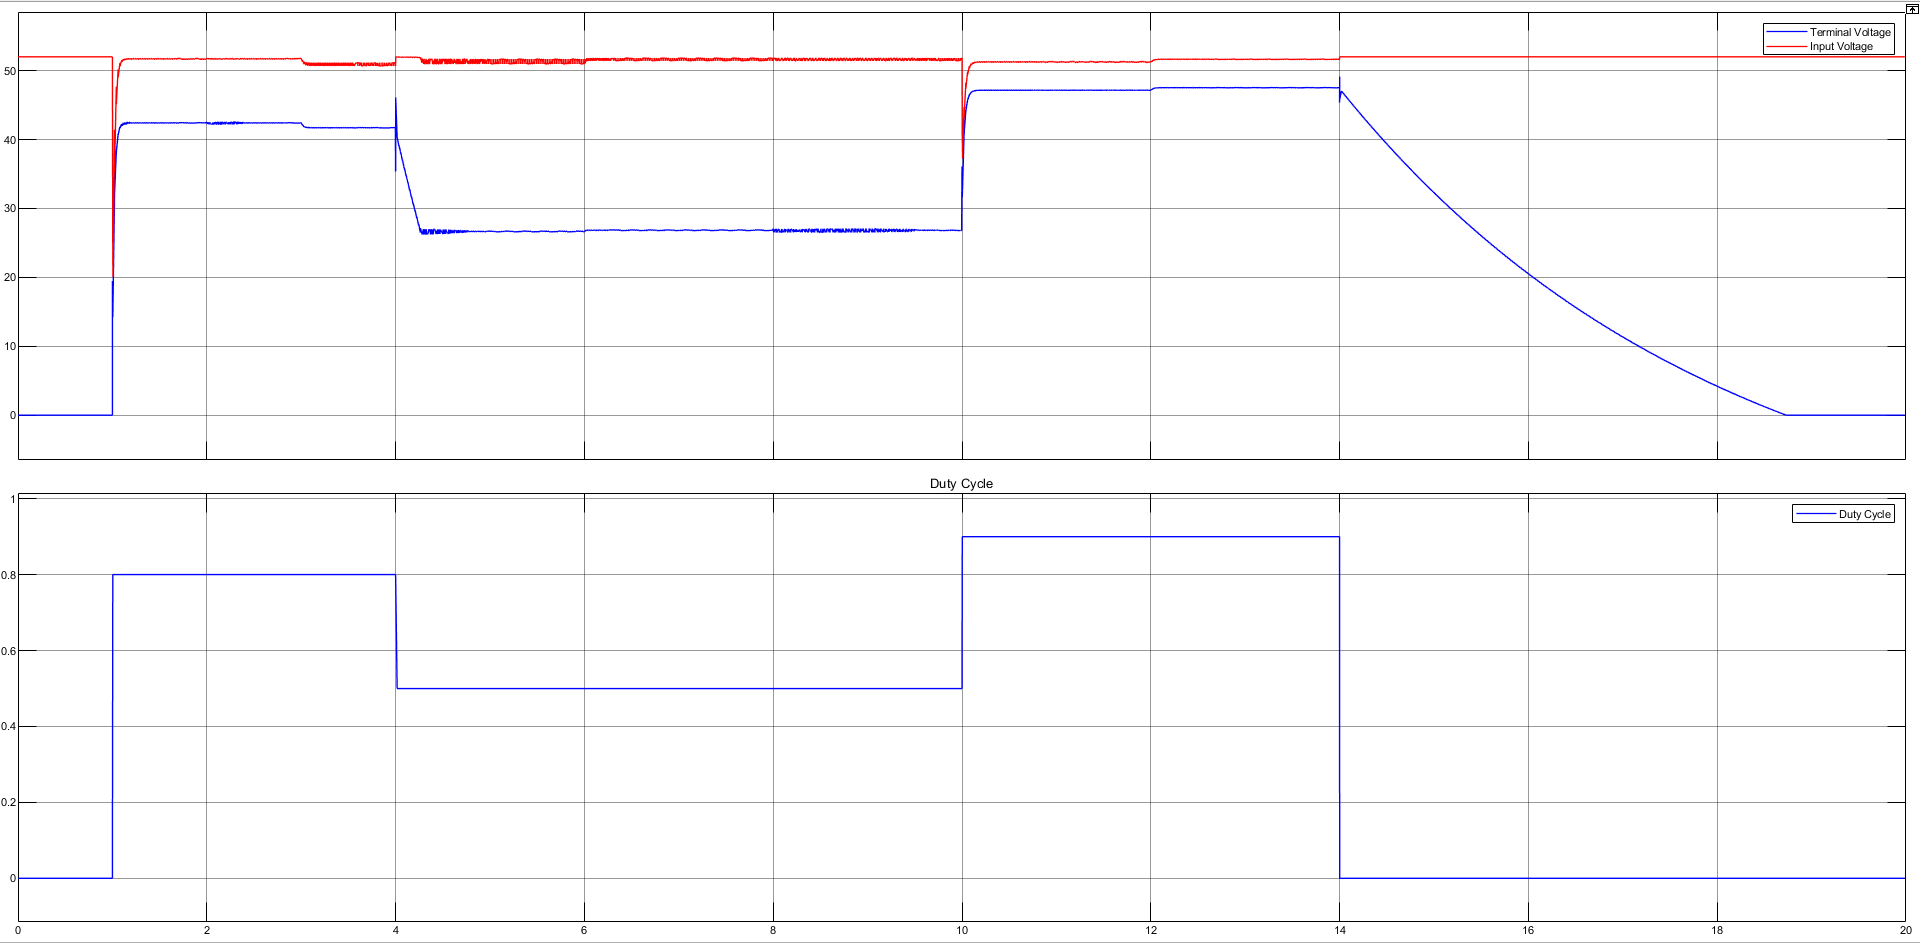
\includegraphics[width=1\textwidth]{case1_2_inputvoltage_terminalvoltage_dutycycle.png}
    \caption{Duty cycle and terminal-input voltages}
    \label{voltages}
\end{figure} 
Terminal voltage is directly proportional to the duty cycle as the duty cycle determines the voltage regulation ratio o the buck converter. We see some sudden drops in the input voltage that is stemmed from the fact explained in part b).
\section{e)}

This case is quite similar to the previous one however here the duty cycle is changed more continiously (a.k.a. no sudden changes). The expected trend is same with the explained in a) except the fact that less overshoot is expected  in this case.
\section{f)}
The plot of currents for case 2 are given in Figure \ref{currents2}.

\begin{figure}[H]
    \centering
    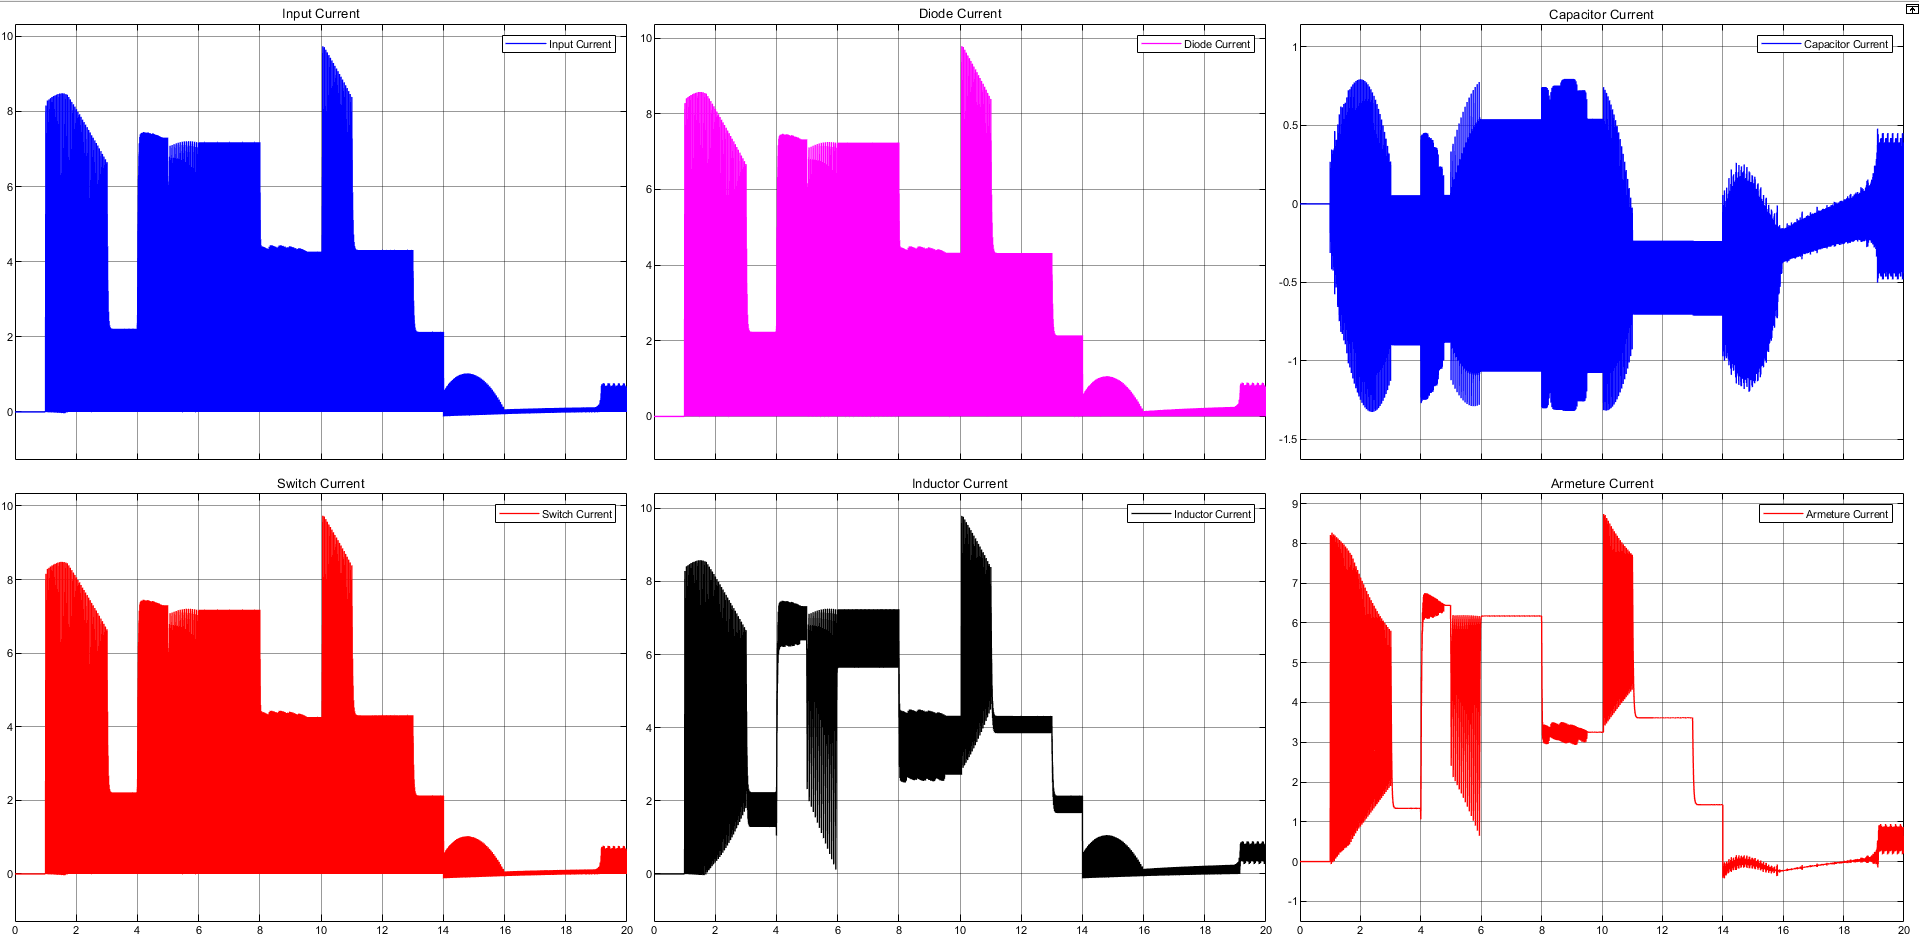
\includegraphics[width=1\textwidth]{case2_1.png}
    \caption{Current plots}
    \label{currents2}
\end{figure} 
So, it can be said that less overshoot is observed. That is, the ripple current because of the switching action became visible in this case. Therefore , the motor is (relatively) soft started.
\section{g)}
The plot that shows the torque data with rotational speed for case 2 is given in Figure \ref{torques2}
\begin{figure}[H]
    \centering
    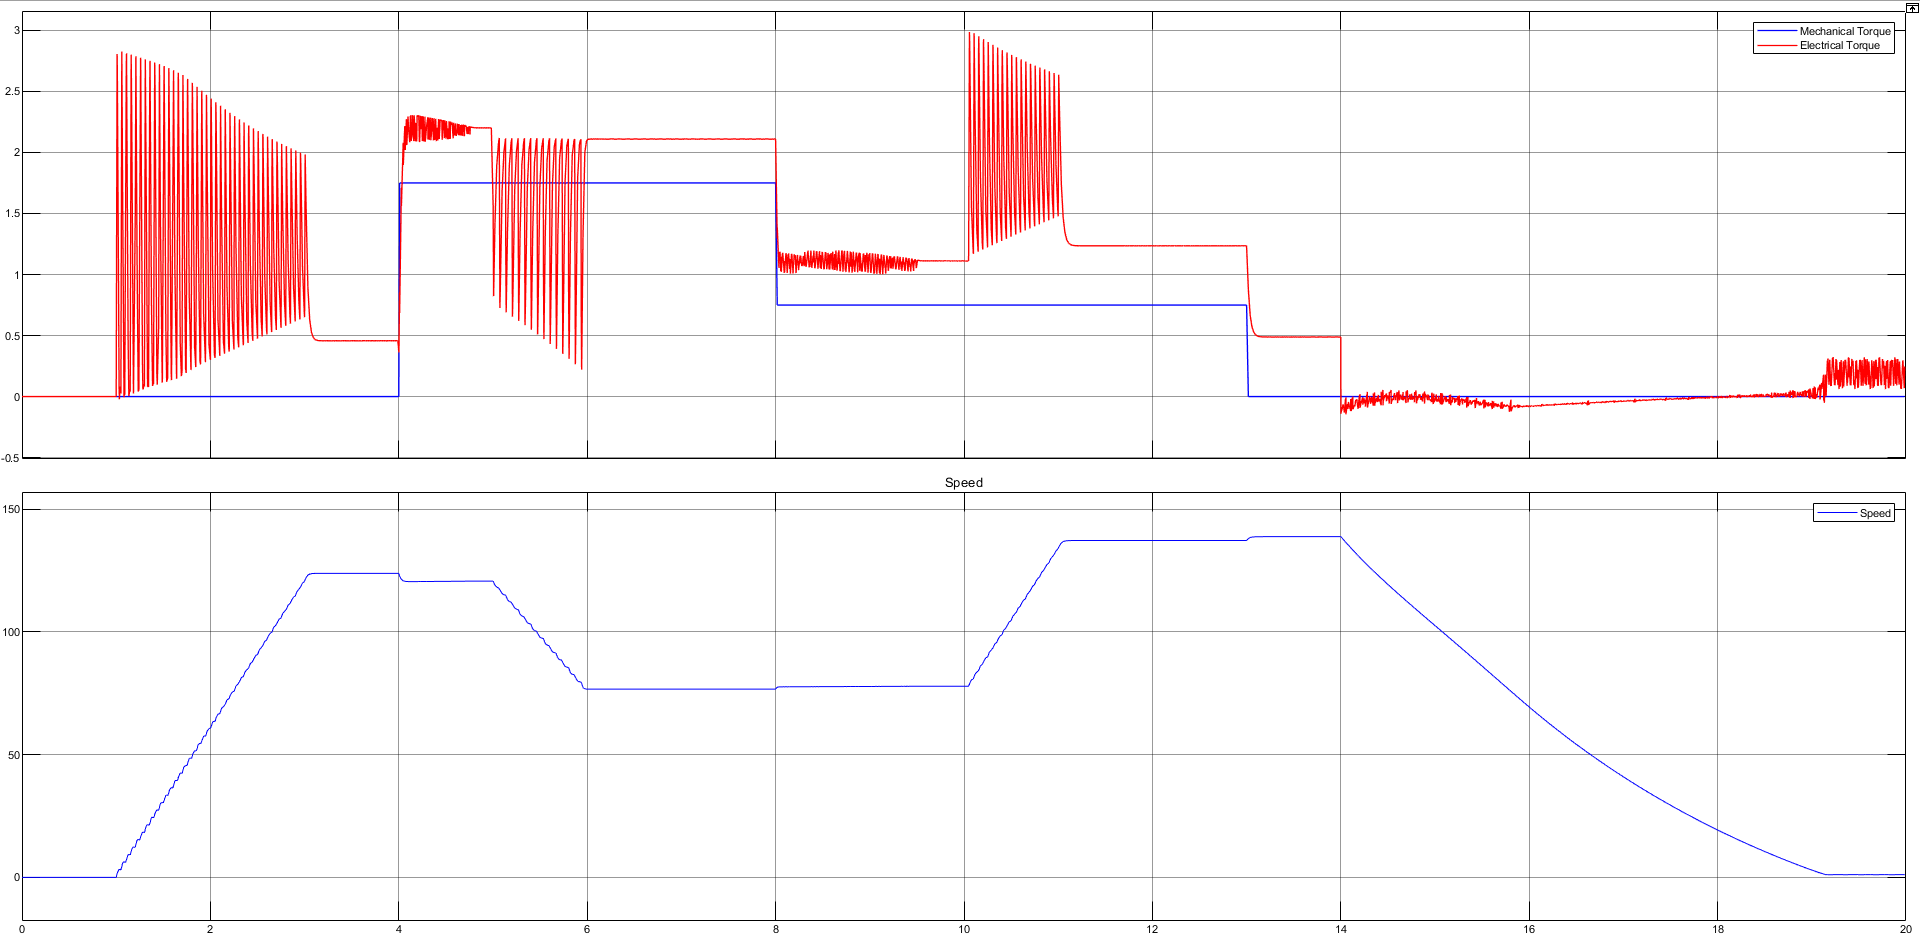
\includegraphics[width=1\textwidth]{case2_2_torque_speed.png}
    \caption{Torque and speed}
    \label{torques2}
\end{figure} 
\section{h)}
The plot that dectribes duty cycle with the input and terminal voltages is given in \ref{voltages2}
\begin{figure}[H]
    \centering
    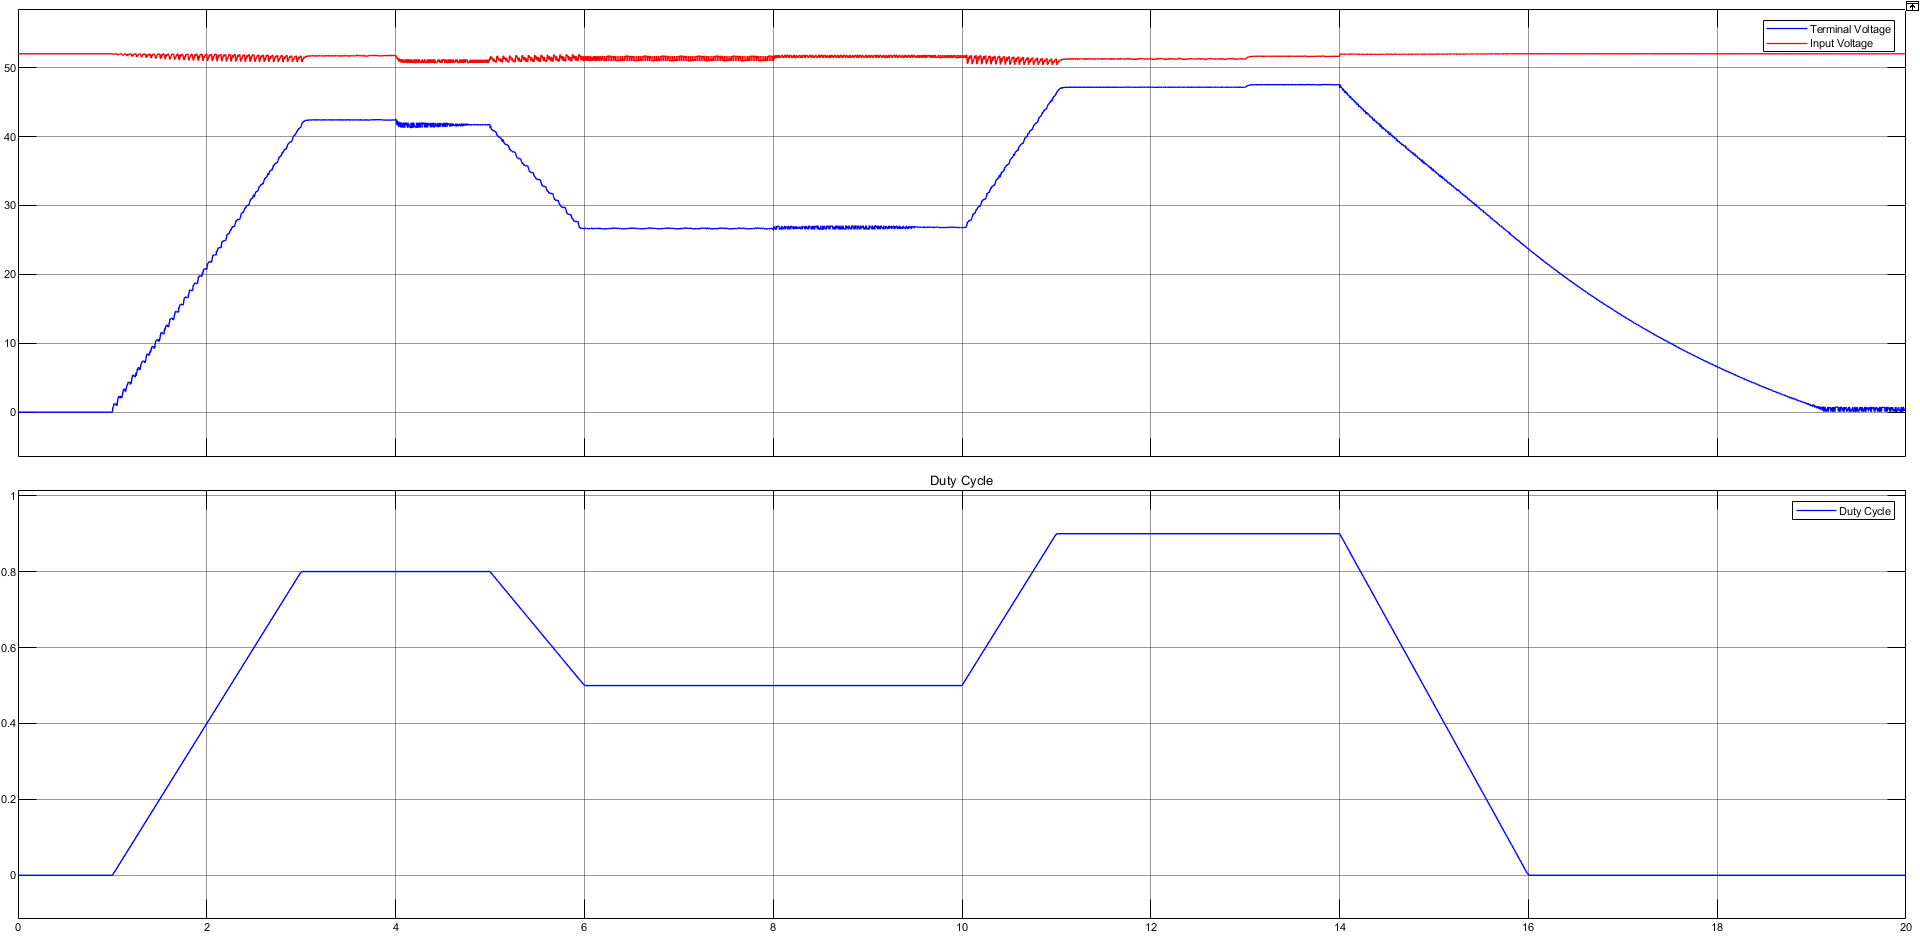
\includegraphics[width=1\textwidth]{case2_2_terminalvoltage-inputvoltage_dutycycle.png}
    \caption{Duty cycle and terminal-input voltages}
    \label{voltages2}
\end{figure} 
\section{i)}
\subsection{A)}
The link between the voltage of a motor and its current is not straightforward. However, the voltage output of the Buck converter, which powers the motor, is associated with the motor's current. The Buck converter is a type of DC-DC converter that lowers the voltage level and its output voltage is regulated by the switching element's duty cycle. This duty cycle is adjusted by a feedback circuit to maintain a consistent output voltage. As the load on the motor increases and the motor current increases, the feedback circuit adjusts the duty cycle to keep the output voltage constant. In summary, the output voltage of the Buck converter that powers the motor is connected to the motor current, but the motor's terminal voltage is not directly linked to it.
\subsection{B)}
The speed of a motor is not determined by its current when the duty cycle is fixed, it is decided by the torque produced and the load on the motor. The torque of a motor depends on the armature and field current, and is inversely proportional to the speed. As the current through the armature and field increases, the torque will increase and cause the motor to speed up, but the load on the motor can also affect the speed. When the duty cycle is fixed, the output voltage and the input voltage to the armature and field winding are fixed, resulting in a fixed current flowing through them. This leads to a fixed torque and a constant speed, not affected by the motor current. The relationship between the speed of a motor and the motor current is not direct when the duty cycle is fixed. The speed is instead decided by the torque produced by the motor and the load on the motor.
\subsection{C)}
While the terminal voltage of a motor is not dependent on the motor current, the motor current is dependent on the terminal voltage. When the load torque remains constant, the current in a DC motor is directly related to the terminal voltage. This is because the terminal voltage is applied to the armature winding of the motor, which produces torque that causes the motor to rotate.
\subsection{D)}
There are various methods that can be employed to prevent the motor current from overshooting when there is a sudden increase in load torque. These include adding a flywheel to increase the load's inertia, using a larger motor for more torque, utilizing a voltage source inverter for precise control of motor voltage, implementing a controller such as PI or PID, using a dynamic braking resistor to absorb surplus energy, and utilizing a DC link capacitor to smooth voltage ripple. The most appropriate approach would depend on the specific system and its requirements. 

\end{document}

%%%%%%%%%%%%%%%%%%%%%%   EXAMPLE TABLE   %%%%%%%%%%%%%%%%%%%%%%%%%%%%%%%%
\begin{table}[H]
\begin{center}
    \caption{Resistance reading by color code convention.}
    \vspace{2mm}
    \begin{tabular}{||c | c | c||} 
        \hline
        Color Order & Value & Tolerance \\ [0.5ex] 
        \hline\hline
        Brown / Black / Red / Gold & 1k\( \Omega \) & \( \% \) 5  \\ 
        \hline
        Yellow / Violet / Red / Gold & 4.7k\( \Omega \) & \( \% \) 5   \\
        \hline
        Brown / Grey / Orange / Gold & 18k\( \Omega \) & \( \% \) 5  \\ [1ex] 
        \hline
    \end{tabular}
\end{center}
\end{table}


%%%%%%%%%%%%%%%%%%%%%%   EXAMPLE IMAGE   %%%%%%%%%%%%%%%%%%%%%%%%%%%%%%%%
\begin{figure}[H]
\centering
\includegraphics[width=1\textwidth]{5.png}
\caption{Circuit schematic for the step 5}
\end{figure} 

%%%%%%%%%%%%%%%%%%%%%%   EXAMPLE IMAGE FROM PDF   %%%%%%%%%%%%%%%%%%%%%%%%%%%%%%%%
\begin{figure}[H] \centering{
	\includegraphics[scale=0.25]{2a_plot.pdf}}
	\caption{Experiment 2}
\end{figure}
	